\section{Auswertung}\label{sec:auswertung}
Im folgenden Kapitel werden die aufgenommenen Messwerte ausgewertet.
\subsection{Überprüfen der Stabilitätsbedingung}
Wie in \autoref{subsubsec:stabilitaet} erläutert, ist Stabilität nur unter der Bedingung $g_1\cdot g_2\in[0,1)$ erfüllt. Für die verwendeten Spiegelkonfigurationen ist dies grafisch in \autoref{fig:stabil} dargestellt.
\begin{figure}[H]
    \centering
    \begin{subfigure}[b]{0.48\textwidth}
        \centering
        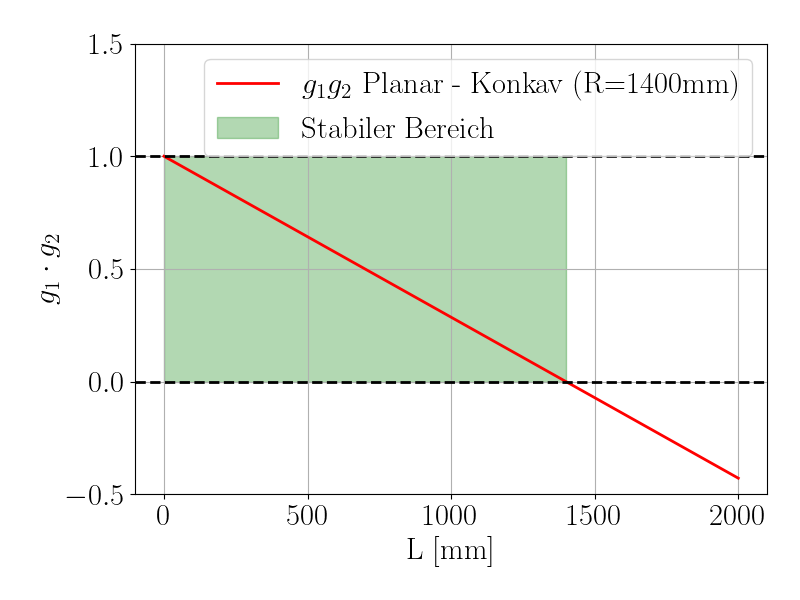
\includegraphics[scale=0.4]{Skripte/2000.png}
        \caption{Konkav-planare Konfiguration}
    \end{subfigure}
    \hfill
    \begin{subfigure}[b]{0.48\textwidth}
        \centering
        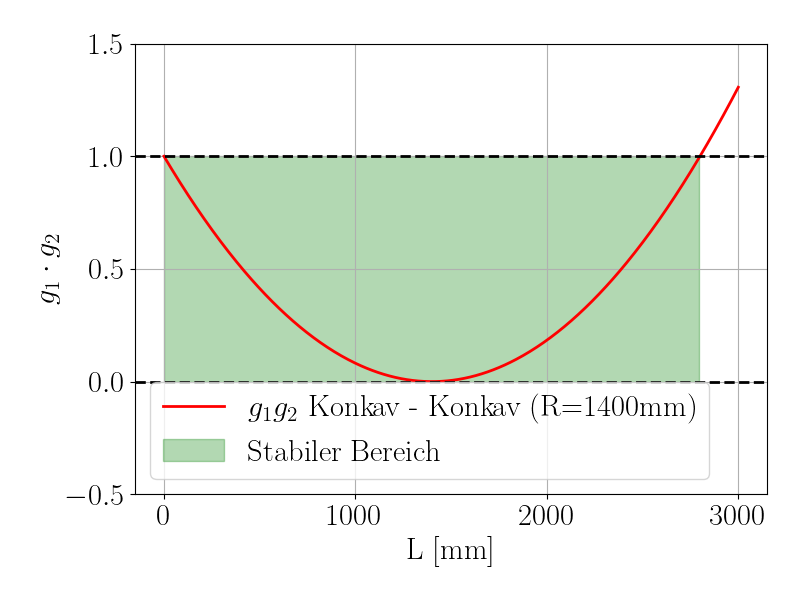
\includegraphics[scale=0.4]{Skripte/3000.png}
        \caption{Konkav-konkave Konfiguration}
    \end{subfigure}
    \caption{Plot der Stabilitätsparameter für verschiedene Resonatorkonfigurationenmit grün hervorgehobenen stabilen Bereich}
    \label{fig:stabil}
\end{figure}
Es ergeben sich die theoretischen Grenzwerte der Resonatorlänge von 
\begin{align}
    L_\text{max k-p}=R=1400
\end{align}
beziehungsweise 
\begin{align}
    L_\text{max k-k}=2\cdot R=2800\text{.}
\end{align}
Im Versuch konnte für den planar-konkaven Resonator eine maximale Länge von \SI{121}{\centi\meter} stabilisiert werden, für die konkav-konkave Kombination wurde die gesamte zur Verfügung stehende Schiene verwendet um eine Resonatorlänge von \SI{218}{\centi\meter} zu erreichen.
\subsubsection{Intensität von TEM-Moden}
Die gemessene Intensität in Abhängigkeit des senkrechten Abstandes zum Strahl ist in \autoref{fig:tem00} dargestellt. Des weiteren ist gemäß der Relation $I(x)=|A(x,y=0,z=const)|^2$ und \autoref{eqn:A} eine Ausgleichfunktion der Form
\begin{align}
    I(x)=\left|C\cdot H_0\left(\sqrt{2}\frac{x+b}{w}\right)\exp{\left(-2\frac{(x+b)^2}{2w^2}\right)}\right|^2
\end{align}
mit den Parametern
\begin{align}
    C &= \SI{3.24(0.01)}{\micro\ampere}\\
    b &= \SI{-0.07(0.04)}{\milli\meter}\\
    w &= \SI{8.47(0.09)}{\milli\meter}\\
\end{align}
bestimmt worden und dargestellt.
\begin{figure}[H]
    \centering
    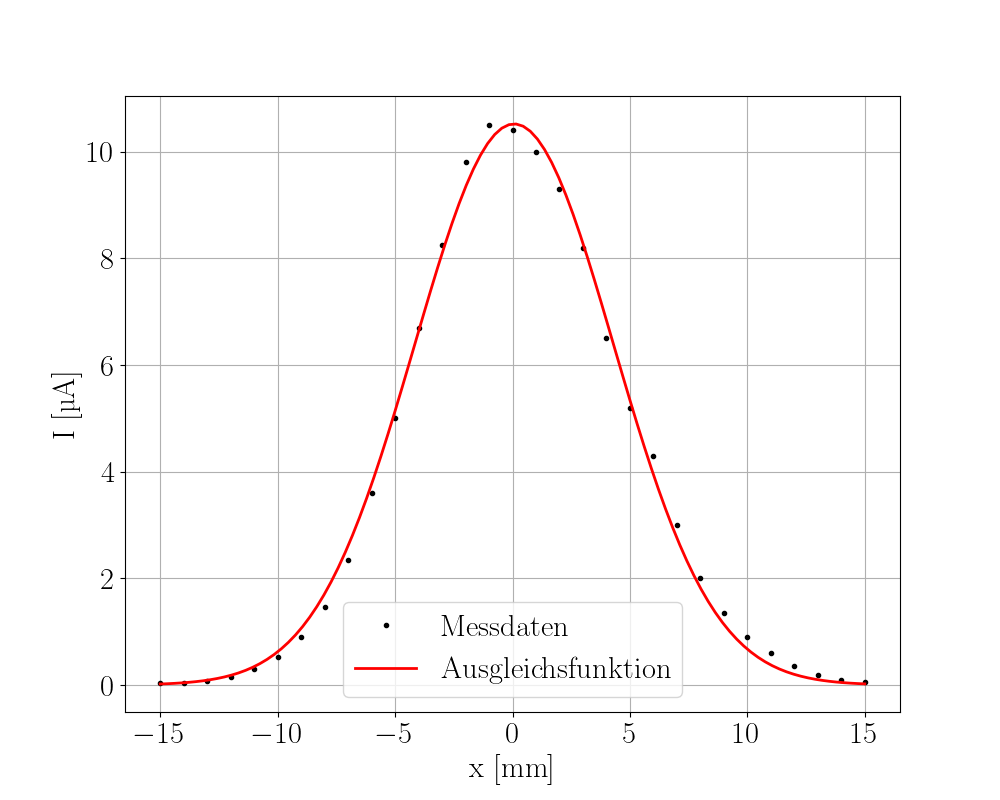
\includegraphics[scale=0.55]{Skripte/TEM00Mode.png}
    \caption{Intensität der $\mathrm{TEM_{00}}$-Mode in gegebener x-Richtung mit Ausgleichfunktion nach \autoref{eqn:A}}\label{fig:tem00}
\end{figure}
Mittels Unterdrückung der $\mathrm{TEM_{00}}$-Mode durch Einschub eines dünnen Drahtes in das Zentrum des Strahls konnte das selbe für die $\mathrm{TEM_{10}}$-Mode durchgeführt werden und die Ausgleichfunktion mit den Parametern
\begin{align}
    C &= \SI{1.39(0.01)}{\micro\ampere}\\
    b &= \SI{-0.77(0.07)}{\milli\meter}\\
    w &= \SI{9.75(0.10)}{\milli\meter}\\
\end{align}
ist zusammen mit den Messwerten in \autoref{fig:tem10} zu sehen.
\begin{figure}[H]
    \centering
    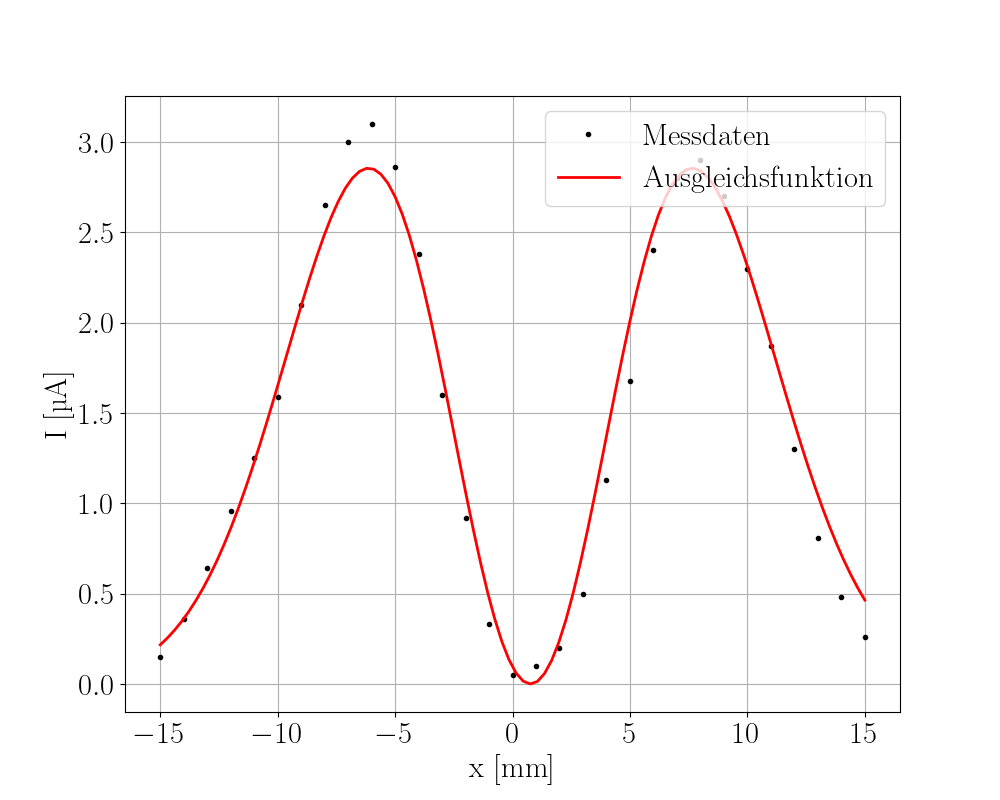
\includegraphics[scale=0.55]{Skripte/TEM10Mode.png}
    \caption{Intensität der $\mathrm{TEM_{10}}$-Mode in gegebener x-Richtung}\label{fig:tem10}
\end{figure}

\subsection{Polarisationsbestimmung}
Die Intensität in Abhängigkeit vom Rotationswinkel des Polarisationsfilters $\alpha$ sind in \autoref{fig:polarisation} zusammen mit einer Ausgleichfunktion der Form
\begin{align}
    I(\alpha)= A\cdot \sin^2{\left(\omega\alpha+\phi\right)}+b
\end{align}
mit den Parametern
\begin{align}
    A &= \SI{3.95(2)}{\micro\ampere} \\
    \omega &= \SI{1.00(0.01)}{\per\radian} \\
    \phi &= \SI{0.39(0.01)}{\radian} \\
    b &= \SI{0.03(0.01)}{\micro\ampere}
\end{align}
dargestellt.
\begin{figure}[H]
    \centering
    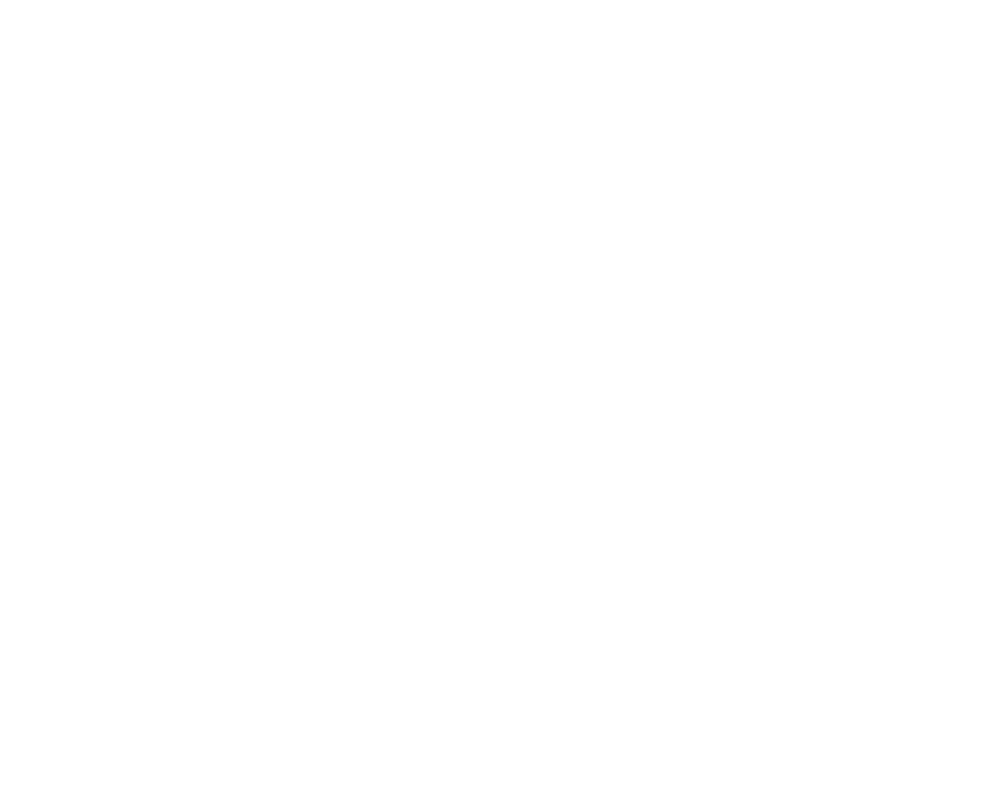
\includegraphics[scale=0.55]{Skripte/polarisation.png}
    \caption{Intensität des Laserstrahls in Abhängigkeit der Polarisationsrichtung}\label{fig:polarisation}
\end{figure}
Die periodische Form der Intensität rührt von dem Einsatz der Brewsterfenster an den Enden des Laserrohrs her, die im Brewster-Winkel zur optischen Achse stehen und das zur Einfallsebene parallel polarisierte Licht an diesen nicht durch Reflexion geschwächt wird. Aufgrund der vielen Umläufe des Lichts im Resonator kann selbst ein geringer Verlust durch Reflexion am Fenster die Entstehung einer Stabilen Mode in der zugehörigen Polarisationsrichtung verhindern.
So ist am niedrigen Wert des Parameters $b$ zu sehen, wie ideal linear das Laserlicht polarisiert ist.
\subsection{Bestimmung der Longitudinalmoden}
\subsection{Ermittlung der Wellenlänge}
Die mittleren Abstände der 1. und 2. Maxima zum Zentrum sind in \autoref{tab:wl} aufgeführt.
\begin{table}[H]
  \centering
  \caption{Gemessene Abstände der Maxima zum Zentrum}
  \label{tab:wl}
  \begin{tabular}{l | l | l}
    \toprule
        {Gitterkonstante $g$ [\si{\micro\meter}]} & {$x_1$ [\si{\centi\meter}]} & {$x_2$ [\si{\centi\meter}]}\\
    \midrule
        80 & 0.416 & 0.850 \\
        100 & 0.350 & 0.650 \\
    \bottomrule
  \end{tabular}
\end{table}
Mit dem Abstand des Gitters zum Schirm $d=\SI{52}{\centi\meter}$ ergibt sich gemäß der Gleichung
\begin{align}
  \lambda\approx\frac{x}{n\cdot d\cdot g}
\end{align} 
für das $n$-te Maximum am Abstand $x$ die Wellenlänge gemittelt als
\begin{align}
  \lambda_\text{gemessen}=\SI{648.0(34.4)}{\nano\meter}\text{.}
\end{align} 